\subsection{exponentiation}

ExponentiationGate is a gate for raising a value to a power. Trace table contains base, bits of the exponent, output, and intermediate value of the bits.

Take $A^{21} = A^{10101_b}$ for example to describe intermediate value, the bits are [1, 0, 1, 0, 1].

\begin{enumerate}
    \item Current bit=1, we start from 1, and times $A^{bit}$ we get $A$
    \item Current bit=0
    \begin{itemize}
        \item Square prev\_intermediate\_value $A^{1_b << 1} = A^{10_b}$
        \item Then times $A^{bit}$ we get $A^{10_b} * A^0 = A^{10_b}$
    \end{itemize}
    \item Current bit=1
    \begin{itemize}
        \item Square prev\_intermediate\_value $A^{10_b<<1} = A^{100_b}$
        \item Then times $A^{bit}$ we get $A^{100_b} * A = A^{101_b}$
    \end{itemize}
    \item Current bit=0
    \begin{itemize}
        \item Square prev\_intermediate\_value $A^{101_b << 1} = A^{1010_b}$
        \item Then times $A^{bit}$ we get $A^{1010_b} * 1 = A^{1010_b}$
    \end{itemize}
    \item Current bit=1
    \begin{itemize}
        \item Square prev\_intermediate\_value $A^{1010_b << 1} = A^{10100_b}$
        \item Then times $A^{bit}$ we get $A^{10100_b} * A = A^{10101_b}$
    \end{itemize}
\end{enumerate}

And we get the last intermediate value $A^{10101_b}$ which should be equal to the output.

Let's take another example of a specific number $2^13 = 2^{1101_b}$, and have a look at the trace cell:
\begin{center}
    \begin{tabular}{ |c|c|c|c|c|c|c|c|c|c| }
        \hline
        base & b\_0 & b\_1 & b\_2 & b\_3 & output & inter\_0 & inter\_1 & inter\_2 & inter\_3 \\
        \hline
        2 & 1 & 0 & 1 & 1 & 8192 & 2 & 8 & 64 & 8192 \\
        \hline
    \end{tabular}
\end{center}

The structure of Gate is shown in the figure:
\begin{figure}[!h]
    \centering
    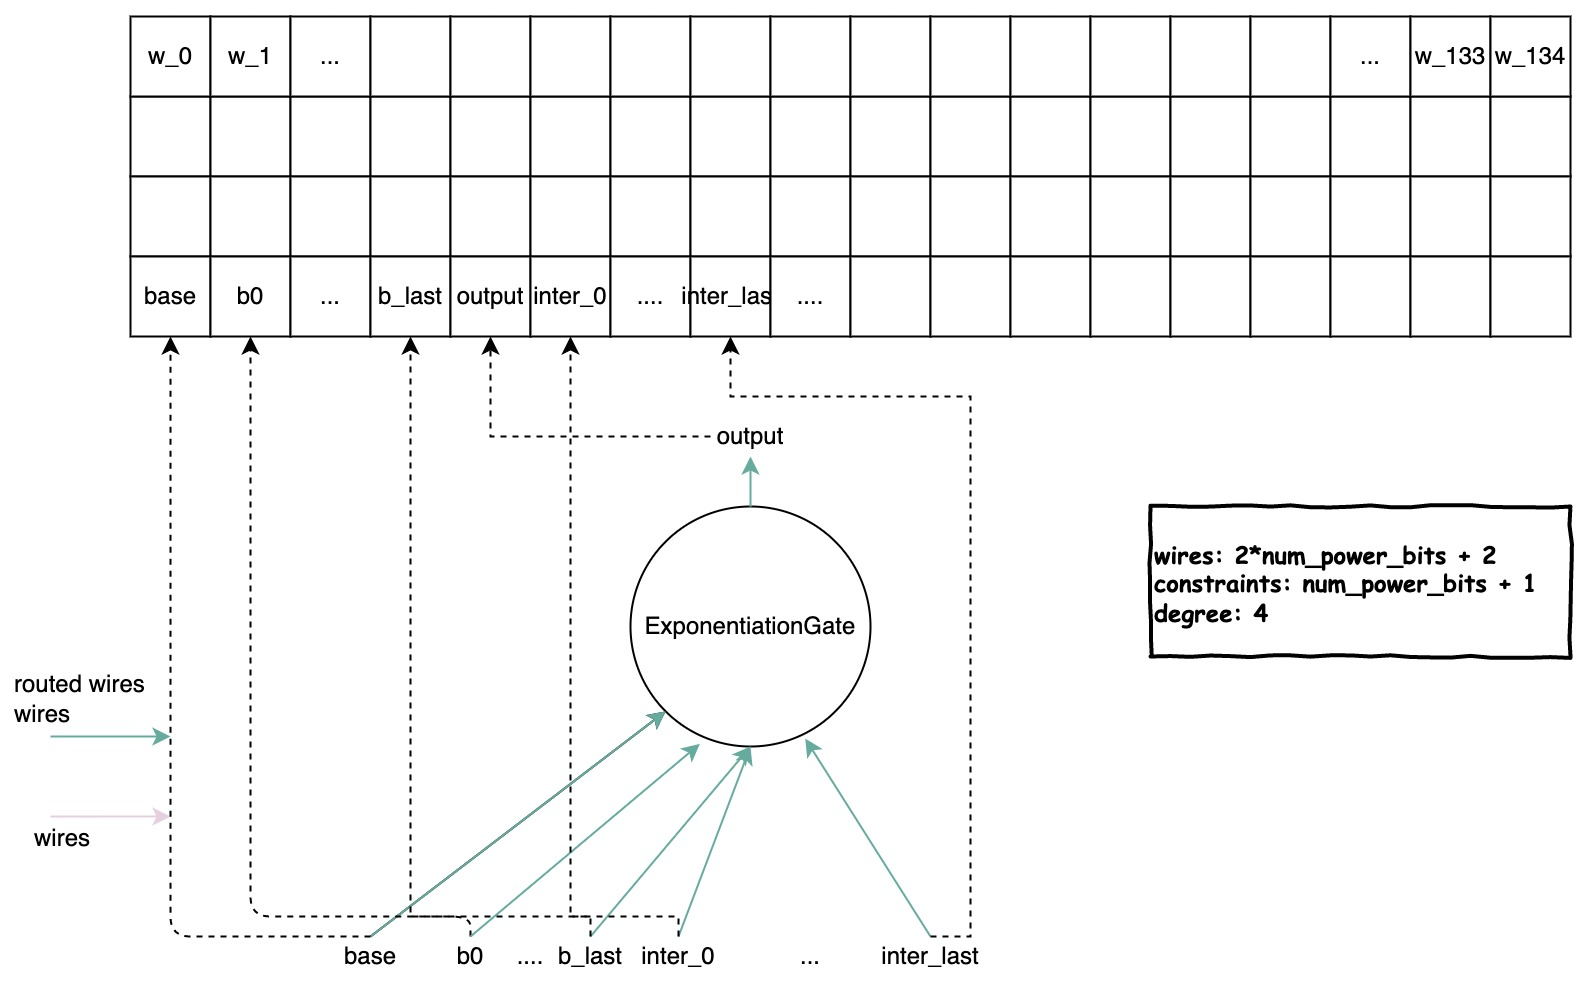
\includegraphics[width=0.8\textwidth]{gates/exponentiation.jpeg}
    \caption{ExponentiationGate}
    \label{fig:exponetiation-gate}
\end{figure}